
%----------------------------------------------------------------------------------------
%	PACKAGES AND OTHER DOCUMENT CONFIGURATIONS
%----------------------------------------------------------------------------------------

\documentclass[11pt,fleqn,oneside]{book} % Default font size and left-justified equations
%----------------------------------------------------------------------------------------
%%%%%%%%%%%%%%%%%%%%%%%%%%%%%%%%%%%%%%%%%
% The Legrand Orange Book
% Structural Definitions File
% Version 2.0 (9/2/15)
%
% Original author:
% Mathias Legrand (legrand.mathias@gmail.com) with modifications by:
% Vel (vel@latextemplates.com)
% 
% This file has been downloaded from:
% http://www.LaTeXTemplates.com
%
% License:
% CC BY-NC-SA 3.0 (http://creativecommons.org/licenses/by-nc-sa/3.0/)
%
%%%%%%%%%%%%%%%%%%%%%%%%%%%%%%%%%%%%%%%%%

%----------------------------------------------------------------------------------------
%	VARIOUS REQUIRED PACKAGES AND CONFIGURATIONS
%----------------------------------------------------------------------------------------

\usepackage[top=3cm,bottom=3cm,left=3cm,right=3cm,headsep=10pt,a4paper]{geometry} % Page margins

\usepackage{graphicx} % Required for including pictures
\graphicspath{{Pictures/}} % Specifies the directory where pictures are stored

\usepackage{lipsum} % Inserts dummy text

\usepackage{tikz} % Required for drawing custom shapes

\usepackage[english]{babel} % English language/hyphenation

\usepackage{enumitem} % Customize lists
\setlist{nolistsep} % Reduce spacing between bullet points and numbered lists

\usepackage{booktabs} % Required for nicer horizontal rules in tables

\usepackage{xcolor} % Required for specifying colors by name
\definecolor{ocre}{RGB}{243,102,25} % Define the orange color used for highlighting throughout the book
\definecolor{darkgoldenrod}{rgb}{0.72, 0.53, 0.04}
\definecolor{gold(metallic)}{rgb}{0.83, 0.69, 0.22}
\definecolor{gold(web)(golden)}{rgb}{1.0, 0.84, 0.0}
\definecolor{goldenbrown}{rgb}{0.6, 0.4, 0.08}
\definecolor{goldenpoppy}{rgb}{0.99, 0.76, 0.0}
\definecolor{goldenyellow}{rgb}{1.0, 0.87, 0.0}
\definecolor{goldenrod}{rgb}{0.85, 0.65, 0.13}
\definecolor{green(colorwheel)(x11green)}{rgb}{0.0, 1.0, 0.0}
\definecolor{green(html/cssgreen)}{rgb}{0.0, 0.5, 0.0}
\definecolor{green(munsell)}{rgb}{0.0, 0.66, 0.47}
\definecolor{green(ryb)}{rgb}{0.4, 0.69, 0.2}
\definecolor{indiagreen}{rgb}{0.07, 0.53, 0.03}
\definecolor{islamicgreen}{rgb}{0.0, 0.56, 0.0}
\definecolor{asparagus}{rgb}{0.53, 0.66, 0.42}
\definecolor{camouflagegreen}{rgb}{0.47, 0.53, 0.42}
\definecolor{airforceblue}{rgb}{0.36, 0.54, 0.66}
\definecolor{silver}{rgb}{0.75, 0.75, 0.75}
\definecolor{trolleygrey}{rgb}{0.5, 0.5, 0.5}
\definecolor{battleshipgrey}{rgb}{0.52, 0.52, 0.51}
\definecolor{cadetgrey}{rgb}{0.57, 0.64, 0.69}
\definecolor{davy\'sgrey}{rgb}{0.33, 0.33, 0.33}
\definecolor{azure(colorwheel)}{rgb}{0.0, 0.5, 1.0}
%----------------------------------------------------------------------------------------
%	FONTS
%----------------------------------------------------------------------------------------

\usepackage{avant} % Use the Avantgarde font for headings
%\usepackage{times} % Use the Times font for headings
\usepackage{mathptmx} % Use the Adobe Times Roman as the default text font together with math symbols from the Sym­bol, Chancery and Com­puter Modern fonts

\usepackage{microtype} % Slightly tweak font spacing for aesthetics
\usepackage[utf8]{inputenc} % Required for including letters with accents
\usepackage[T1]{fontenc} % Use 8-bit encoding that has 256 glyphs

%----------------------------------------------------------------------------------------
%	BIBLIOGRAPHY AND INDEX
%----------------------------------------------------------------------------------------

\usepackage[style=numeric,citestyle=numeric,sorting=nyt,sortcites=true,autopunct=true,babel=hyphen,hyperref=true,abbreviate=false,backref=true,backend=biber]{biblatex}
\addbibresource{bibliography.bib} % BibTeX bibliography file
\defbibheading{bibempty}{}

\usepackage{calc} % For simpler calculation - used for spacing the index letter headings correctly
\usepackage{makeidx} % Required to make an index
\makeindex % Tells LaTeX to create the files required for indexing

%----------------------------------------------------------------------------------------
%	MAIN TABLE OF CONTENTS
%----------------------------------------------------------------------------------------

\usepackage{titletoc} % Required for manipulating the table of contents

\contentsmargin{0cm} % Removes the default margin

% Part text styling
\titlecontents{part}[0cm]
{\addvspace{20pt}\centering\large\bfseries}
{}
{}
{}

% Chapter text styling
\titlecontents{chapter}[1.25cm] % Indentation
{\addvspace{12pt}\large\sffamily\bfseries} % Spacing and font options for chapters
{\color{trolleygrey!60}\contentslabel[\Large\thecontentslabel]{1.25cm}\color{trolleygrey}} % Chapter number
{\color{trolleygrey}}  
{\color{trolleygrey!60}\normalsize\;\titlerule*[.5pc]{.}\;\thecontentspage} % Page number

% Section text styling 
\titlecontents{section}[1.75cm] % Indentation
{\addvspace{3pt}\sffamily\bfseries} % Spacing and font options for sections
{\color{battleshipgrey!60}\contentslabel[\thecontentslabel]{1.25cm}\color{battleshipgrey}} % Section number
{\color{battleshipgrey}}  
{\color{battleshipgrey!60}\titlerule*[.5pc]{.}\;\thecontentspage} % Page number
[]

% Subsection text styling 
\titlecontents{subsection}[2.25cm] % Indentation
{\addvspace{1pt}\sffamily\small} % Spacing and font options for subsections
{\color{cadetgrey!60}\contentslabel[\thecontentslabel]{1.25cm}\color{cadetgrey}} % Subsection number
{\color{cadetgrey}}  
{\hfill\color{cadetgrey!60}\thecontentspage} % Page number
[]

% List of figures
\titlecontents{figure}[0em]
{\addvspace{-5pt}\sffamily}
{\thecontentslabel\hspace*{1em}}
{}
{\ \titlerule*[.5pc]{.}\;\thecontentspage}
[]

% List of tables
\titlecontents{table}[0em]
{\addvspace{-5pt}\sffamily}
{\thecontentslabel\hspace*{1em}}
{}
{\ \titlerule*[.5pc]{.}\;\thecontentspage}
[]

%----------------------------------------------------------------------------------------
%	MINI TABLE OF CONTENTS IN PART HEADS
%----------------------------------------------------------------------------------------

% Chapter text styling
\titlecontents{lchapter}[0em] % Indenting
{\addvspace{15pt}\large\sffamily\bfseries} % Spacing and font options for chapters
{\color{trolleygrey}\contentslabel[\Large\thecontentslabel]{1.25cm}\color{trolleygrey}} % Chapter number
{}  
{\color{trolleygrey}\normalsize\sffamily\bfseries\;\titlerule*[.5pc]{.}\;\thecontentspage} % Page number

% Section text styling
\titlecontents{lsection}[0em] % Indenting
{\sffamily\small} % Spacing and font options for sections
{\contentslabel[\thecontentslabel]{1.25cm}} % Section number
{}
{}

% Subsection text styling
\titlecontents{lsubsection}[.5em] % Indentation
{\normalfont\footnotesize\sffamily} % Font settings
{}
{}
{}

%----------------------------------------------------------------------------------------
%	PAGE HEADERS
%----------------------------------------------------------------------------------------

\usepackage{fancyhdr} % Required for header and footer configuration

\pagestyle{fancy}
\renewcommand{\chaptermark}[1]{\markboth{\sffamily\normalsize\bfseries\chaptername\ \thechapter.\ #1}{}} % Chapter text font settings
\renewcommand{\sectionmark}[1]{\markright{\sffamily\normalsize\thesection\hspace{5pt}#1}{}} % Section text font settings
\fancyhf{} \fancyhead[LE,RO]{\sffamily\normalsize\thepage} % Font setting for the page number in the header
\fancyhead[LO]{\rightmark} % Print the nearest section name on the left side of odd pages
\fancyhead[RE]{\leftmark} % Print the current chapter name on the right side of even pages
\renewcommand{\headrulewidth}{0.5pt} % Width of the rule under the header
\addtolength{\headheight}{2.5pt} % Increase the spacing around the header slightly
\renewcommand{\footrulewidth}{0pt} % Removes the rule in the footer
\fancypagestyle{plain}{\fancyhead{}\renewcommand{\headrulewidth}{0pt}} % Style for when a plain pagestyle is specified

% Removes the header from odd empty pages at the end of chapters
\makeatletter
% 
% \renewcommand{\cleardoublepage}{
% \clearpage\ifodd\c@page\else
% \hbox{}
% \vspace*{\fill}
% \thispagestyle{empty}
% \newpage
% \fi}

%----------------------------------------------------------------------------------------
%	THEOREM STYLES
%----------------------------------------------------------------------------------------

\usepackage{amsmath,amsfonts,amssymb,amsthm} % For math equations, theorems, symbols, etc

\newcommand{\intoo}[2]{\mathopen{]}#1\,;#2\mathclose{[}}
\newcommand{\ud}{\mathop{\mathrm{{}d}}\mathopen{}}
\newcommand{\intff}[2]{\mathopen{[}#1\,;#2\mathclose{]}}
\newtheorem{notation}{Notation}[chapter]

% Boxed/framed environments
\newtheoremstyle{ocrenumbox}% % Theorem style name
{0pt}% Space above
{0pt}% Space below
{\normalfont}% % Body font
{}% Indent amount
{\small\bf\sffamily\color{trolleygrey}}% % Theorem head font
{\;}% Punctuation after theorem head
{0.25em}% Space after theorem head
{\small\sffamily\color{trolleygrey}\thmname{#1}\nobreakspace\thmnumber{\@ifnotempty{#1}{}\@upn{#2}}% Theorem text (e.g. Theorem 2.1)
\thmnote{\nobreakspace\the\thm@notefont\sffamily\bfseries\color{black}---\nobreakspace#3.}} % Optional theorem note
\renewcommand{\qedsymbol}{$\blacksquare$}% Optional qed square

\newtheoremstyle{blacknumex}% Theorem style name
{5pt}% Space above
{5pt}% Space below
{\normalfont}% Body font
{} % Indent amount
{\small\bf\sffamily}% Theorem head font
{\;}% Punctuation after theorem head
{0.25em}% Space after theorem head
{\small\sffamily{\tiny\ensuremath{\blacksquare}}\nobreakspace\thmname{#1}\nobreakspace\thmnumber{\@ifnotempty{#1}{}\@upn{#2}}% Theorem text (e.g. Theorem 2.1)
\thmnote{\nobreakspace\the\thm@notefont\sffamily\bfseries---\nobreakspace#3.}}% Optional theorem note

\newtheoremstyle{blacknumbox} % Theorem style name
{0pt}% Space above
{0pt}% Space below
{\normalfont}% Body font
{}% Indent amount
{\small\bf\sffamily}% Theorem head font
{\;}% Punctuation after theorem head
{0.25em}% Space after theorem head
{\small\sffamily\thmname{#1}\nobreakspace\thmnumber{\@ifnotempty{#1}{}\@upn{#2}}% Theorem text (e.g. Theorem 2.1)
\thmnote{\nobreakspace\the\thm@notefont\sffamily\bfseries---\nobreakspace#3.}}% Optional theorem note

% Non-boxed/non-framed environments
\newtheoremstyle{ocrenum}% % Theorem style name
{5pt}% Space above
{5pt}% Space below
{\normalfont}% % Body font
{}% Indent amount
{\small\bf\sffamily\color{trolleygrey}}% % Theorem head font
{\;}% Punctuation after theorem head
{0.25em}% Space after theorem head
{\small\sffamily\color{trolleygrey}\thmname{#1}\nobreakspace\thmnumber{\@ifnotempty{#1}{}\@upn{#2}}% Theorem text (e.g. Theorem 2.1)
\thmnote{\nobreakspace\the\thm@notefont\sffamily\bfseries\color{black}---\nobreakspace#3.}} % Optional theorem note
\renewcommand{\qedsymbol}{$\blacksquare$}% Optional qed square
\makeatother

% Defines the theorem text style for each type of theorem to one of the three styles above
\newcounter{dummy} 
\numberwithin{dummy}{section}
\theoremstyle{ocrenumbox}
\newtheorem{theoremeT}[dummy]{Theorem}
\newtheorem{problem}{Problem}[chapter]
\newtheorem{exerciseT}{Exercise}[chapter]
\theoremstyle{blacknumex}
\newtheorem{exampleT}{Example}[chapter]
\theoremstyle{blacknumbox}
\newtheorem{vocabulary}{Vocabulary}[chapter]
\newtheorem{definitionT}{Definition}[section]
\newtheorem{corollaryT}[dummy]{Corollary}
\theoremstyle{ocrenum}
\newtheorem{proposition}[dummy]{Proposition}

%----------------------------------------------------------------------------------------
%	DEFINITION OF COLORED BOXES
%----------------------------------------------------------------------------------------

\RequirePackage[framemethod=default]{mdframed} % Required for creating the theorem, definition, exercise and corollary boxes

% Theorem box
\newmdenv[skipabove=7pt,
skipbelow=7pt,
backgroundcolor=black!5,
linecolor=trolleygrey,
innerleftmargin=5pt,
innerrightmargin=5pt,
innertopmargin=5pt,
leftmargin=0cm,
rightmargin=0cm,
innerbottommargin=5pt]{tBox}

% Exercise box	  
\newmdenv[skipabove=7pt,
skipbelow=7pt,
rightline=false,
leftline=true,
topline=false,
bottomline=false,
backgroundcolor=trolleygrey!10,
linecolor=trolleygrey,
innerleftmargin=5pt,
innerrightmargin=5pt,
innertopmargin=5pt,
innerbottommargin=5pt,
leftmargin=0cm,
rightmargin=0cm,
linewidth=4pt]{eBox}	

% Definition box
\newmdenv[skipabove=7pt,
skipbelow=7pt,
rightline=false,
leftline=true,
topline=false,
bottomline=false,
linecolor=trolleygrey,
innerleftmargin=5pt,
innerrightmargin=5pt,
innertopmargin=0pt,
leftmargin=0cm,
rightmargin=0cm,
linewidth=4pt,
innerbottommargin=0pt]{dBox}	

% Corollary box
\newmdenv[skipabove=7pt,
skipbelow=7pt,
rightline=false,
leftline=true,
topline=false,
bottomline=false,
linecolor=gray,
backgroundcolor=black!5,
innerleftmargin=5pt,
innerrightmargin=5pt,
innertopmargin=5pt,
leftmargin=0cm,
rightmargin=0cm,
linewidth=4pt,
innerbottommargin=5pt]{cBox}

% Creates an environment for each type of theorem and assigns it a theorem text style from the "Theorem Styles" section above and a colored box from above
\newenvironment{theorem}{\begin{tBox}\begin{theoremeT}}{\end{theoremeT}\end{tBox}}
\newenvironment{exercise}{\begin{eBox}\begin{exerciseT}}{\hfill{\color{trolleygrey}\tiny\ensuremath{\blacksquare}}\end{exerciseT}\end{eBox}}				  
\newenvironment{definition}{\begin{dBox}\begin{definitionT}}{\end{definitionT}\end{dBox}}	
\newenvironment{example}{\begin{exampleT}}{\hfill{\tiny\ensuremath{\blacksquare}}\end{exampleT}}		
\newenvironment{corollary}{\begin{cBox}\begin{corollaryT}}{\end{corollaryT}\end{cBox}}	

%----------------------------------------------------------------------------------------
%	REMARK ENVIRONMENT
%----------------------------------------------------------------------------------------

\newenvironment{remark}{\par\vspace{10pt}\small % Vertical white space above the remark and smaller font size
\begin{list}{}{
\leftmargin=35pt % Indentation on the left
\rightmargin=25pt}\item\ignorespaces % Indentation on the right
\makebox[-2.5pt]{\begin{tikzpicture}[overlay]
\node[draw=trolleygrey!60,line width=1pt,circle,fill=trolleygrey!25,font=\sffamily\bfseries,inner sep=2pt,outer sep=0pt] at (-15pt,0pt){\textcolor{trolleygrey}{R}};\end{tikzpicture}} % Orange R in a circle
\advance\baselineskip -1pt}{\end{list}\vskip5pt} % Tighter line spacing and white space after remark

%----------------------------------------------------------------------------------------
%	SECTION NUMBERING IN THE MARGIN
%----------------------------------------------------------------------------------------

\makeatletter
\renewcommand{\@seccntformat}[1]{\llap{\textcolor{trolleygrey}{\csname the#1\endcsname}\hspace{1em}}}                    
\renewcommand{\section}{\@startsection{section}{1}{\z@}
{-4ex \@plus -1ex \@minus -.4ex}
{1ex \@plus.2ex }
{\normalfont\LARGE\sffamily\bfseries\textcolor{trolleygrey}}}
\renewcommand{\subsection}{\@startsection {subsection}{2}{\z@}
{-3ex \@plus -0.1ex \@minus -.4ex}
{0.5ex \@plus.2ex }
{\normalfont\Large\sffamily\bfseries\textcolor{battleshipgrey}}}
\renewcommand{\subsubsection}{\@startsection {subsubsection}{3}{\z@}
{-2ex \@plus -0.1ex \@minus -.2ex}
{.2ex \@plus.2ex }
{\normalfont\sffamily\bfseries}}                        
\renewcommand\paragraph{\@startsection{paragraph}{4}{\z@}
{-2ex \@plus-.2ex \@minus .2ex}
{.1ex}
{\normalfont\small\sffamily\bfseries}}

%----------------------------------------------------------------------------------------
%	PART HEADINGS
%----------------------------------------------------------------------------------------

% numbered part in the table of contents
\newcommand{\@mypartnumtocformat}[2]{%
\setlength\fboxsep{0pt}%
\noindent\colorbox{trolleygrey!20}{\strut\parbox[c][.7cm]{\ecart}{\color{trolleygrey!70}\Large\sffamily\bfseries\centering#1}}\hskip\esp\colorbox{trolleygrey!40}{\strut\parbox[c][.7cm]{\linewidth-\ecart-\esp}{\Large\sffamily\centering#2}}}%
%%%%%%%%%%%%%%%%%%%%%%%%%%%%%%%%%%
% unnumbered part in the table of contents
\newcommand{\@myparttocformat}[1]{%
\setlength\fboxsep{0pt}%
\noindent\colorbox{trolleygrey!40}{\strut\parbox[c][.7cm]{\linewidth}{\Large\sffamily\centering#1}}}%
%%%%%%%%%%%%%%%%%%%%%%%%%%%%%%%%%%
\newlength\esp
\setlength\esp{4pt}
\newlength\ecart
\setlength\ecart{1.2cm-\esp}
\newcommand{\thepartimage}{}%
\newcommand{\partimage}[1]{\renewcommand{\thepartimage}{#1}}%
\def\@part[#1]#2{%
\ifnum \c@secnumdepth >-2\relax%
\refstepcounter{part}%
\addcontentsline{toc}{part}{\texorpdfstring{\protect\@mypartnumtocformat{\thepart}{#1}}{\partname~\thepart\ ---\ #1}}
\else%
\addcontentsline{toc}{part}{\texorpdfstring{\protect\@myparttocformat{#1}}{#1}}%
\fi%
\startcontents%
\markboth{}{}%
{\thispagestyle{empty}%
\begin{tikzpicture}[remember picture,overlay]%
\node at (current page.north west){\begin{tikzpicture}[remember picture,overlay]%	
\fill[trolleygrey!20](0cm,0cm) rectangle (\paperwidth,-\paperheight);
\node[anchor=north] at (4cm,-3.25cm){\color{trolleygrey!40}\fontsize{220}{100}\sffamily\bfseries\thepart}; 
\node[anchor=south east] at (\paperwidth-1cm,-\paperheight+1cm){\parbox[t][][t]{8.5cm}{
\printcontents{l}{0}{\setcounter{tocdepth}{1}}%
}};
\node[anchor=north east] at (\paperwidth-1.5cm,-3.25cm){\parbox[t][][t]{15cm}{\strut\raggedleft\color{white}\fontsize{30}{30}\sffamily\bfseries#2}};
\end{tikzpicture}};
\end{tikzpicture}}%
\@endpart}
\def\@spart#1{%
\startcontents%
\phantomsection
{\thispagestyle{empty}%
\begin{tikzpicture}[remember picture,overlay]%
\node at (current page.north west){\begin{tikzpicture}[remember picture,overlay]%	
\fill[trolleygrey!20](0cm,0cm) rectangle (\paperwidth,-\paperheight);
\node[anchor=north east] at (\paperwidth-1.5cm,-3.25cm){\parbox[t][][t]{15cm}{\strut\raggedleft\color{white}\fontsize{30}{30}\sffamily\bfseries#1}};
\end{tikzpicture}};
\end{tikzpicture}}
\addcontentsline{toc}{part}{\texorpdfstring{%
\setlength\fboxsep{0pt}%
\noindent\protect\colorbox{trolleygrey!40}{\strut\protect\parbox[c][.7cm]{\linewidth}{\Large\sffamily\protect\centering #1\quad\mbox{}}}}{#1}}%
\@endpart}
\def\@endpart{\vfil\newpage
\if@twoside
\if@openright
\null
\thispagestyle{empty}%
\newpage
\fi
\fi
\if@tempswa
\twocolumn
\fi}

%----------------------------------------------------------------------------------------
%	CHAPTER HEADINGS
%----------------------------------------------------------------------------------------

% A switch to conditionally include a picture, implemented by  Christian Hupfer
\newif\ifusechapterimage
\usechapterimagetrue
\newcommand{\thechapterimage}{}%
\newcommand{\chapterimage}[1]{\ifusechapterimage\renewcommand{\thechapterimage}{#1}\fi}%
\newcommand{\autodot}{.}
\def\@makechapterhead#1{%
{\parindent \z@ \raggedright \normalfont
\ifnum \c@secnumdepth >\m@ne
\if@mainmatter
\begin{tikzpicture}[remember picture,overlay]
\node at (current page.north west)
{\begin{tikzpicture}[remember picture,overlay]
\node[anchor=north west,inner sep=0pt] at (0,0) {\ifusechapterimage\includegraphics[width=\paperwidth]{\thechapterimage}\fi};
\ifusechapterimage
    \draw[anchor=west] (\Gm@lmargin,-6.5cm) node [line width=2pt,rounded corners=15pt,draw=azure(colorwheel),fill=white,fill opacity=0.9,inner sep=15pt]{\strut\makebox[22cm]{}};
    \draw[anchor=west] (\Gm@lmargin+.3cm,-6.5cm) node {\huge\sffamily\bfseries\color{trolleygrey}\thechapter\autodot~#1\strut};
\else
    \draw[anchor=west] (\Gm@lmargin,-3.5cm) node [line width=2pt,rounded corners=15pt,draw=azure(colorwheel),fill=white,fill opacity=0.9,inner sep=15pt]{\strut\makebox[22cm]{}};
    \draw[anchor=west] (\Gm@lmargin+.3cm,-3.5cm) node {\huge\sffamily\bfseries\color{trolleygrey}\thechapter\autodot~#1\strut};
\fi
\end{tikzpicture}};
\end{tikzpicture}
\else
\begin{tikzpicture}[remember picture,overlay]
\node at (current page.north west)
{\begin{tikzpicture}[remember picture,overlay]
\node[anchor=north west,inner sep=0pt] at (0,0) {\ifusechapterimage\includegraphics[width=\paperwidth]{\thechapterimage}\fi};
\ifusechapterimage
    \draw[anchor=west] (\Gm@lmargin,-6.5cm) node [line width=2pt,rounded corners=15pt,draw=azure(colorwheel),fill=white,fill opacity=0.9,inner sep=15pt]{\strut\makebox[22cm]{}};
    \draw[anchor=west] (\Gm@lmargin+.3cm,-6.5cm) node {\huge\sffamily\bfseries\color{trolleygrey}#1\strut};
\else
    \draw[anchor=west] (\Gm@lmargin,-3.5cm) node [line width=2pt,rounded corners=15pt,draw=azure(colorwheel),fill=white,fill opacity=0.9,inner sep=15pt]{\strut\makebox[22cm]{}};
    \draw[anchor=west] (\Gm@lmargin+.3cm,-3.5cm) node {\huge\sffamily\bfseries\color{trolleygrey}#1\strut};
\fi
\end{tikzpicture}};
\end{tikzpicture}
\fi\fi
\ifusechapterimage
    \par\vspace*{180\p@}
\else
    \par\vspace*{120\p@}
\fi
}}

%-------------------------------------------

\def\@makeschapterhead#1{%
\begin{tikzpicture}[remember picture,overlay]
\node at (current page.north west)
{\begin{tikzpicture}[remember picture,overlay]
\node[anchor=north west,inner sep=0pt] at (0,0) {\ifusechapterimage\includegraphics[width=\paperwidth]{\thechapterimage}\fi};
\ifusechapterimage
    \draw[anchor=west] (\Gm@lmargin,-6.5cm) node [line width=2pt,rounded corners=15pt,draw=azure(colorwheel),fill=white,fill opacity=0.9,inner sep=15pt]{\strut\makebox[22cm]{}};
    \draw[anchor=west] (\Gm@lmargin+.3cm,-6.5cm) node {\huge\sffamily\bfseries\color{trolleygrey}#1\strut};
\else
    \draw[anchor=west] (\Gm@lmargin,-3.5cm) node [line width=2pt,rounded corners=15pt,draw=azure(colorwheel),fill=white,fill opacity=0.9,inner sep=15pt]{\strut\makebox[22cm]{}};
    \draw[anchor=west] (\Gm@lmargin+.3cm,-3.5cm) node {\huge\sffamily\bfseries\color{trolleygrey}#1\strut};
\fi
\end{tikzpicture}};
\end{tikzpicture}
\ifusechapterimage
    \par\vspace*{180\p@}
\else
    \par\vspace*{120\p@}
\fi
}
\makeatother

%----------------------------------------------------------------------------------------
%	HYPERLINKS IN THE DOCUMENTS
%----------------------------------------------------------------------------------------

\usepackage{hyperref}
\hypersetup{hidelinks,backref=true,pagebackref=true,hyperindex=true,colorlinks=false,breaklinks=true,urlcolor= trolleygrey,bookmarks=true,bookmarksopen=false,pdftitle={Title},pdfauthor={Author}}
\usepackage{bookmark}
\bookmarksetup{
open,
numbered,
addtohook={%
\ifnum\bookmarkget{level}=0 % chapter
\bookmarksetup{bold}%
\fi
\ifnum\bookmarkget{level}=-1 % part
\bookmarksetup{color=trolleygrey,bold}%
\fi
}
}
 % Insert the commands.tex file which contains the majority of the structure behind the template
\begin{document}

%----------------------------------------------------------------------------------------
%	TITLE PAGE
%----------------------------------------------------------------------------------------
\begingroup
\thispagestyle{empty}
\begin{tikzpicture}[remember picture,overlay]
    \node(background) at (current page.center) {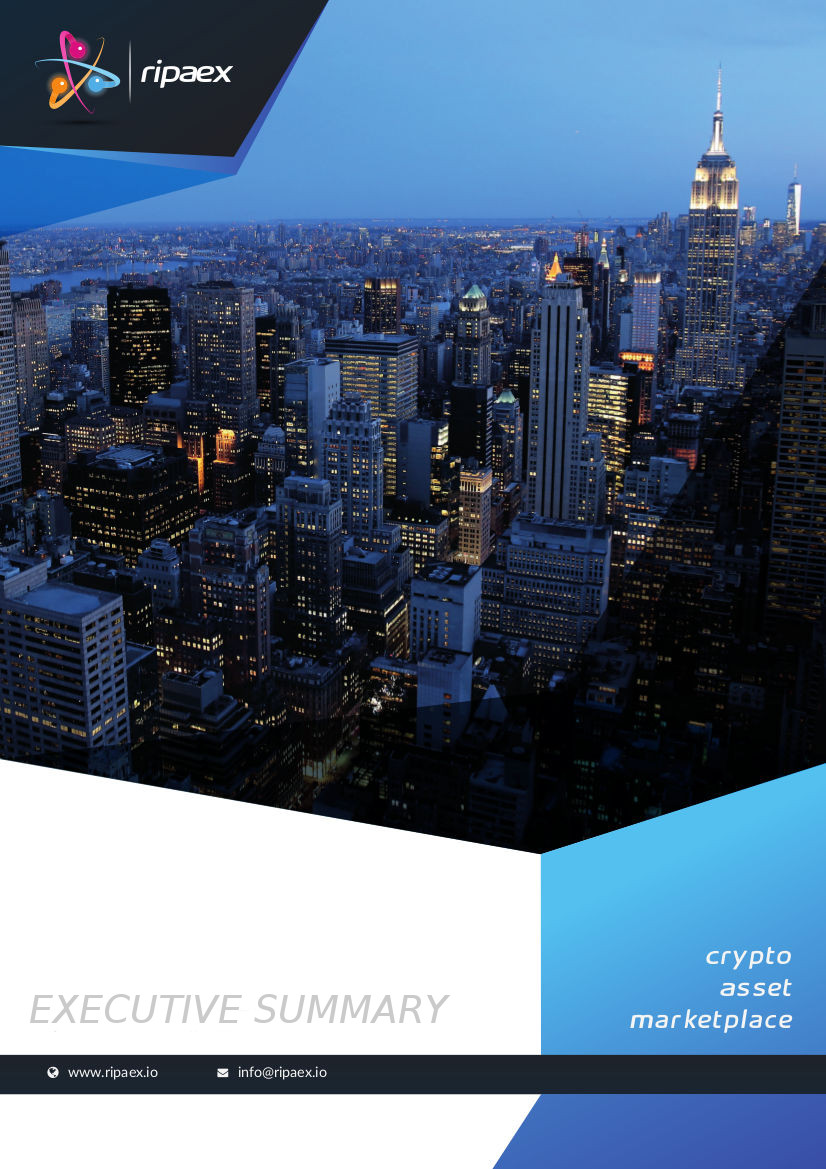
\includegraphics[height=\paperheight]{backgroundES}};
\end{tikzpicture}
\endgroup

% \begingroup
% \section{Abstract}\index{Abstract}
% \thispagestyle{empty}
% \addcontentsline{toc}{chapter}{\textcolor{trolleygrey}{Abstract}}
\pagestyle{empty} % No headers
\usechapterimagefalse % If you don't want to include a chapter image, use this to toggle images off - it can be enabled later with \usechapterimagetrue
\chapter{Abstract}
\textbf{Ripa Exchange is a hybrid-decentralized exchange with a strong focus on lowering the entry level
of opening new exchanges and giving crypto traders safe and secure trading partners to operate on a daily basis.}\\

The team of RipaEx believes that, despite the recent developments in the world of
cryptocurrencies, it is still expensive to open, manage and build trust on a newly created exchange not
only for the resources need to run a reliable exchange platform but also for the build of the platform 
itself and to find the liquidity necessary to run a profitable business in the first 5 years gap.\\

Action is needed and action is needed now. Users are frustrated with unreliable exchanges that run away
with their funds, got hacked or does not sustain the load of a growing industry of today. Despite
the effort of exchanges managers to offer efficient, reliable, and easy to use platforms to trade entry
prices for building such platforms is in the rage of 250-300 thousand euro and that does not 
include personnel cost to give platinum customer support, platform infrastructure and daily expenses for
the business. All of that for then having an decent exchange platform for which you will need to pay an 
external software company to make changes as you request.\\

It is the aim of this project to give you an Open Source, efficient, reliable exchange platform and to
give the needed liquidity\footnote{Thank you to the RLSP (Ripa Liquidity Service Provider) technology} to your newly created 
exchange from day \textbf{one} so you can focus on finding your customers, give platinum support and comply with all the heterogeneous 
laws in the industry. 
As we want that the customer experience will be the sleekest possible, while making it safer to trade.\\
\usechapterimagetrue
% \endgroup


%----------------------------------------------------------------------------------------
%	CHAPTER 2: Introduction
%----------------------------------------------------------------------------------------

\chapterimage{chapter_head_2_London.jpg} % Chapter heading image

\chapter{Introduction}

\section{Key Terminology}
	\begin{description}
		\item[\textsc{Ripa Exchange:}] a FIAT $\Leftrightarrow$ CRYPTO exchange (a cryptocurrency exchange) based on the source code
		of Peatio \cite{peatio}
		\item[\textsc{Ripa Blockchain:}] a DPOS blockchain in which liquidity is shared for all the exchanges in the Ripa network
		\item[\textsc{Ripa Token - XPX:}] a cryptographically secure token exchanged on the Ripa blockchain based on the DPOS protocol
		\item[\textsc{RIPA:}] the DPOS financial ecosystem composed of Ripa Exchange and Ripa Blockchain
		\item[\textsc{RIPAEX:}] the name of the project, project website and hosted domain
		\item[\textsc{RLSP:}] Ripa Liquidity Service Provider, a shared orderbook to exchange orders and liquidity between exchanges in the same Ripa network
		\item[\textsc{RipaEx ICO:}] the name of fixed exchange rate token exchange period composed of both the phases of PreSale and RIPA TEC
		\item[\textsc{ARK:}] a platform for consumer adoption of blockchain technologies \cite{ark}
		\item[\textsc{ACES:}] Ark Contract Execution Services \cite{aces} provides simple protocols and tools for building a robust 
		blockchain service marketplace based on the ARK SmartBridge technology
		\item[\textsc{``,'' or ``.'':}] The Anglo-Saxon use of decimal points and commas to represent numbers has
		been chosen for the purposes of this document: that is to say that a “.” represents a decimal point, and a “,”
		distinguishes between multiples of thousands, millions and billions.
    \end{description}

%\pagebreak
\section{Roadmap}
There are essentially four phases to the RipaEx project:
\tcbset{roadmapBox/.style={colback=yellow!10!white,colframe=azure(colorwheel),
equal height group=nobefaf,width=(\linewidth-1pt), height from=4cm to 8cm, nobeforeafter,
	center title,
	valign=top, halign=left}}
\begin{center}
	\begin{tcolorbox}[roadmapBox,
		title=\textbf{\textsc{Funding the project: XPX PreSale and RIPA TEC (WP2)}}]

		This phase recognizes the existence of interest in this market development
		from across the World concerning the lowering of the entry level for building a cryptocurrency exchange.
		It aims to make the first comprehensive analysis of this state of the art to form the basis of the later project phases and
		build the first working prototype of a centralized exchange based on Peatio.\\
		\vspace{1cm}
		\centering\textbf{\textsc{Phase ending January 2019}}.
	\end{tcolorbox}
	\resizebox{0.05\textwidth}{26pt}{$\Downarrow$}
	\begin{tcolorbox}[roadmapBox,
		title=\textbf{\textsc{First exchange opening and development of tools and resources (WP3)}}]

		The second phase takes the results of the first 
		and develops from them a set of tools and resources which provide concise and comprehensible guidance to market actors in any
		Country. With the first instance of Ripa Exchange running we can make first contact with other economical players in the industry.\\
		\vspace{1cm}
		\centering\textbf{\textsc{Phase ending June 2019}}.
	\end{tcolorbox}
	\resizebox{0.05\textwidth}{26pt}{$\Downarrow$}
	\begin{tcolorbox}[roadmapBox,
		title=\textbf{\textsc{Dissemination (WP 7/8) and Project Coordination (WP1)}}]

		During the full duration of the project, 
		dissemination activities (WP 7/8) are carried out in which results from the individual work packages are disseminated 
		to relevant target groups including project partners, RipaEx investors, exchanges managers, banking partners as well 
		as relevant target groups. This phase covers a wide range of dissemination techniques, from printed and
		electronic handbooks to workshops and training sessions, hackatons, ongoing networks, all having the
		ultimate goal of defining a standard for exchange communication among public and private entities. 
		An overarching work package is concerned with the management of the project from start to finish, 
		ensuring proper coordination, quality assurance and budgetary control (WP1).
	\end{tcolorbox}
	\resizebox{0.05\textwidth}{26pt}{$\Downarrow$}
	\begin{tcolorbox}[roadmapBox,
		title=\textbf{\textsc{Development of hybrid-decentralized exchange (WP 4-6)}}]

		Using the tools and resources developed in WP3, 
		Work packages 4-6 focus on bringing collected knowledge and tools into practice. The three work packages reflect three major
		focal points (and target groups) within the network of exchanges created for establishing successful 
		demonstrations on a local scale: incorporations of local Ripa Exchanges (WP4), technical analysis for the 
		Ripa Liquidity Service Provider (WP5), and first MVP of the hybrid decentralized exchange (WP6). The demonstration
		phase forms the heart of the RipaEx action; WP 2 and 3 are focused on providing
		deliverables (e.g. tools) that enable successful and efficient demonstration activities.\\
		\vspace{1cm}
		\centering\textbf{\textsc{Phase ending January 2021}}.
	\end{tcolorbox}
\end{center}

\section{RipaEx Governance}\index{RipaEx Governance}
Creation of a new Ripa Exchange in the Ripa network, release of RCF funds for the creation of new exchanges will be
decided with a majority voting system among all the delegates of the Ripa network. The customization of the individual
exchange instance, otherwise, will be decided exclusively from the company that manages that single exchange
instance.

The RipaEx project will be incorporated as a collective interest company for profit as soon as the Ripa Blockchain
will be stable, instead the company Ripa Exchange Ltd will manage the first individual crypto asset marketplace
instance that will be opened to public in the first quarter of 2019.

%----------------------------------------------------------------------------------------
%	CHAPTER 3: Ripa Exchange
%----------------------------------------------------------------------------------------

\chapterimage{chapter_head_3_Singapore.jpg} % Chapter heading image

\chapter{Ripa Exchange - Ripa Blockchain}

\section{Mission}
\begin{quotation}
	``\textit{Our mission is to build the world best open source crypto asset marketplace with a high performance trading engine 
	and safety which can be trusted and enjoyed by users. Additionally we want to move the crypto currency exchange technology 
	forward by providing support and add new features. We are helping people to build easy their own exchange around the world.}''
\end{quotation}

Help is greatly appreciated, feel free to submit pull-requests or open issues in our \href{https://github.com/RipaEx}{GitHub repositories}.

\section{The Ripa Exchange}
\subsection{Features}
A free, transparent and internationalized open source crypto currency exchange.

\tcbset{featureBox/.style={colback=yellow!10!white,colframe=white!20!black,
equal height group=nobefaf,width=(\linewidth-1pt)/3, height=5.0cm, nobeforeafter,
	center title,
	valign=top, halign=left}}
\begin{tcolorbox}[featureBox,
	title=\textsc{Open Source} \faCircleONotch]

	\small	All source code are fully released under the terms of the MIT License.\\\vspace{5mm}
	\tiny Ripa Exchange is a customizable cryptocurrency exchange solution architecture enables easy connection to KYC/AML, 
	authentication, ETL/reporting, and other services.
\end{tcolorbox}
\begin{tcolorbox}[featureBox,
	title=\textsc{Compliant} \faCheck]

	\small	International KYC/AML standards.\\\vspace{5mm}
	\tiny Ripa Exchange KYC efficiently submits and exchanges KYC information 
	to meet the banking supervisory standards and comply with Customer Due Diligence (CDD) requirements.
\end{tcolorbox}
\begin{tcolorbox}[featureBox,
	title=\textsc{Transparent \& Configurable} \faCogs]

	\small	Customize in your own way\\\vspace{5mm}
	\tiny Major functions have been embedded in the source code – neat registration and log-in interface, 
	personalized deposit and withdraw procedure, best match of bid and ask, etc. These functions are comprehensive 
	and are ready to use with no extra work needed. 
\end{tcolorbox}

\begin{tcolorbox}[featureBox,
	title=\textsc{Internationalization} \faLanguage]

	\small	All users are able to view Ripa Exchange in a language to their best convenience.\\\vspace{5mm}
	\tiny Supporting many common languages, Ripa Exchange makes it easy for users to operate in their mother tongue. 
	You are encouraged to contribute to our language variety. Users will benefit from your efforts.
\end{tcolorbox}
\begin{tcolorbox}[featureBox,
	title=\textsc{Proof of Solvency} \faUsers]

	\small	Easy deployable PoS.\\\vspace{5mm}
	\tiny Ripa Exchange Proof of Solvency (PoS) allows users to verify 
	the solvency of the Ripa Exchange based cryptocurrency exchange without compromising user privacy.
\end{tcolorbox}
\begin{tcolorbox}[featureBox,
	title=\textsc{Multi-Accounts Trading} \faHandSpockO]

	\small	Easy currency configuration.\\\vspace{5mm}
	\tiny Ripa Exchange allows to create multiple accounts and trading in multiple currencies. 
	Ripa Exchange makes it is easy to trade different currencies.
\end{tcolorbox}

\begin{tcolorbox}[featureBox,
	title=\textsc{Multi-Accounts Users} \faSuitcase]

	\small	Easy account configuration.\\\vspace{5mm}
	\tiny Ripa Exchange allows to create multiple login accounts Google, Facebook, Twitter and FIDO Alliance
	login standards to secure your account.
\end{tcolorbox}
\begin{tcolorbox}[featureBox,
	title=\textsc{Enterprise Exchange} \faInstitution]

	\small	Start small, grow big.\\\vspace{5mm}
	\tiny Ripa Exchange enterprise exchange features include a high-performance matching engine, 
	scalable distributed worker threads, and SMS 2-factor authentication.
\end{tcolorbox}
\begin{tcolorbox}[featureBox,
	title=\textsc{Functional \& Intuitive} \faIntersex]

	\small	For the new trader, for the experienced trader.\\\vspace{5mm}
	\tiny Clean, user friendly registration and login interface. 
	Personalized deposit and withdraw procedure and a built-in proof-of-solvency audit.
\end{tcolorbox}

\subsection{Features at Launch}
At the first working Ripa Exchange instance opening the following features will be functioning:
\begin{itemize}
	\item \textsc{CRYPTO $\Leftrightarrow$ CRYPTO}:
	\item \textsc{OAuth}: Facebook, Google, Twitter
	\item \textsc{FIDO}: login with FIDO Alliance standards
	\item \textsc{Protocols}: POW, DPOS, Masternode, tether, ERC20
	\item \textsc{Currencies}: BTC, ETH, DOGE, BCH, TUSD, ARK, LISK, SHIFT, RISE, KAPU, OXY, RIPA, promising ERC20 tokens
	\item \textsc{Main Markets}: BTC, ETH, ARK
	\item \textsc{Orders Type}: market, limit
\end{itemize}

\section{The Ripa Blockchain}
The RipaEx project will have its own blockchain called Ripa which will be run on the DPOS protocol and has the XPX 
token (\PHP symbol) running on it that will serve the five following purposes:
	\begin{enumerate}
		\item to list new cryptocurrencies on Ripa Exchanges
		\item to advertise new projects
		\item to buy RipaEx gadget on the RipaEx Store
		\item to pay for the sell of goods \& services on authorized resellers with our RipaEx POS (Point of Sale)
		\item to share liquidity between Ripa Exchanges in the same network
	\end{enumerate}

\subsection{Delegated Proof of Stake Technology}
Ripa Blockchain, will inherits the Delegated Proof of Stake (DPoS) consensus system that was first introduced
by BitShares. This consensus algorithm was designed to eliminate the issues associated with Proof of Work (PoW), 
namely the centralization of computing power and the exponentially increasing waste of real world energy. While not
completely decentralized as it relies on consensus by a fixed number of elected delegates, it guarantees a better decentralization 
than Bitcoin. The consensus algorithm implementation is improved over time, evolving into an optimal consensus system.\\

The technical description of the Ripa blockchain is as follow:
\begin{enumerate}
	\item DPoS (Delegated Proof of Stake)
	\begin{itemize}
		\item 101 active forging Delegates
		\item Delegates selected by vote mechanism built into DPoS
		\item 115,000,000 XPX - Seeded Genesis Block
	\end{itemize}
	\item Multi-signature accounts
	\item Constant block reward
	\begin{itemize}
		\item 2 \PHP per block
		\item Inflation Rate (with 8s block times)
		\begin{itemize}
			\item 6.31\% for the first year
			\item 5.93\% the 2nd year
			\item 4.02\% the 10th year
		\end{itemize}
		\item 8-second block time
		\begin{itemize}
			\item Decreased block time possible with future upgrades to the core.
		\end{itemize}
		\item 25 transactions per block
		\begin{itemize}
			\item Increased via soft fork as needed.
		\end{itemize}
	\end{itemize}
	\item Routing tables
	\item SmartBridge data field for custom use and bridging blockchains (ARK Contract Execution Service)
	\item Batch transactions\footnote{Future upgrade: when ARK 2.0 will be released \label{note1}}
	\item Custom transaction fees\footnotemark[\value{footnote}]
	\item Native smart contract execution\footnote{Future upgrade: when ARK Virtual Machine will be released}
\end{enumerate}

\subsection{Connecting Blockchains}
\subsubsection{ARK Bridged Blockchains (SmartBridge Technology)}
The ARK Platform does not provide direct support for sidechains or dapp databases.
Instead, a mechanism to bridge together blockchains is provided via a bridging
function built into ARK Core where any blockchain can send and receive trigger
function notices and informational data through the primary ARK network via
custom developed \textbf{SmartBridge(s)} and \textbf{Encoded Listeners}.
\begin{center}
	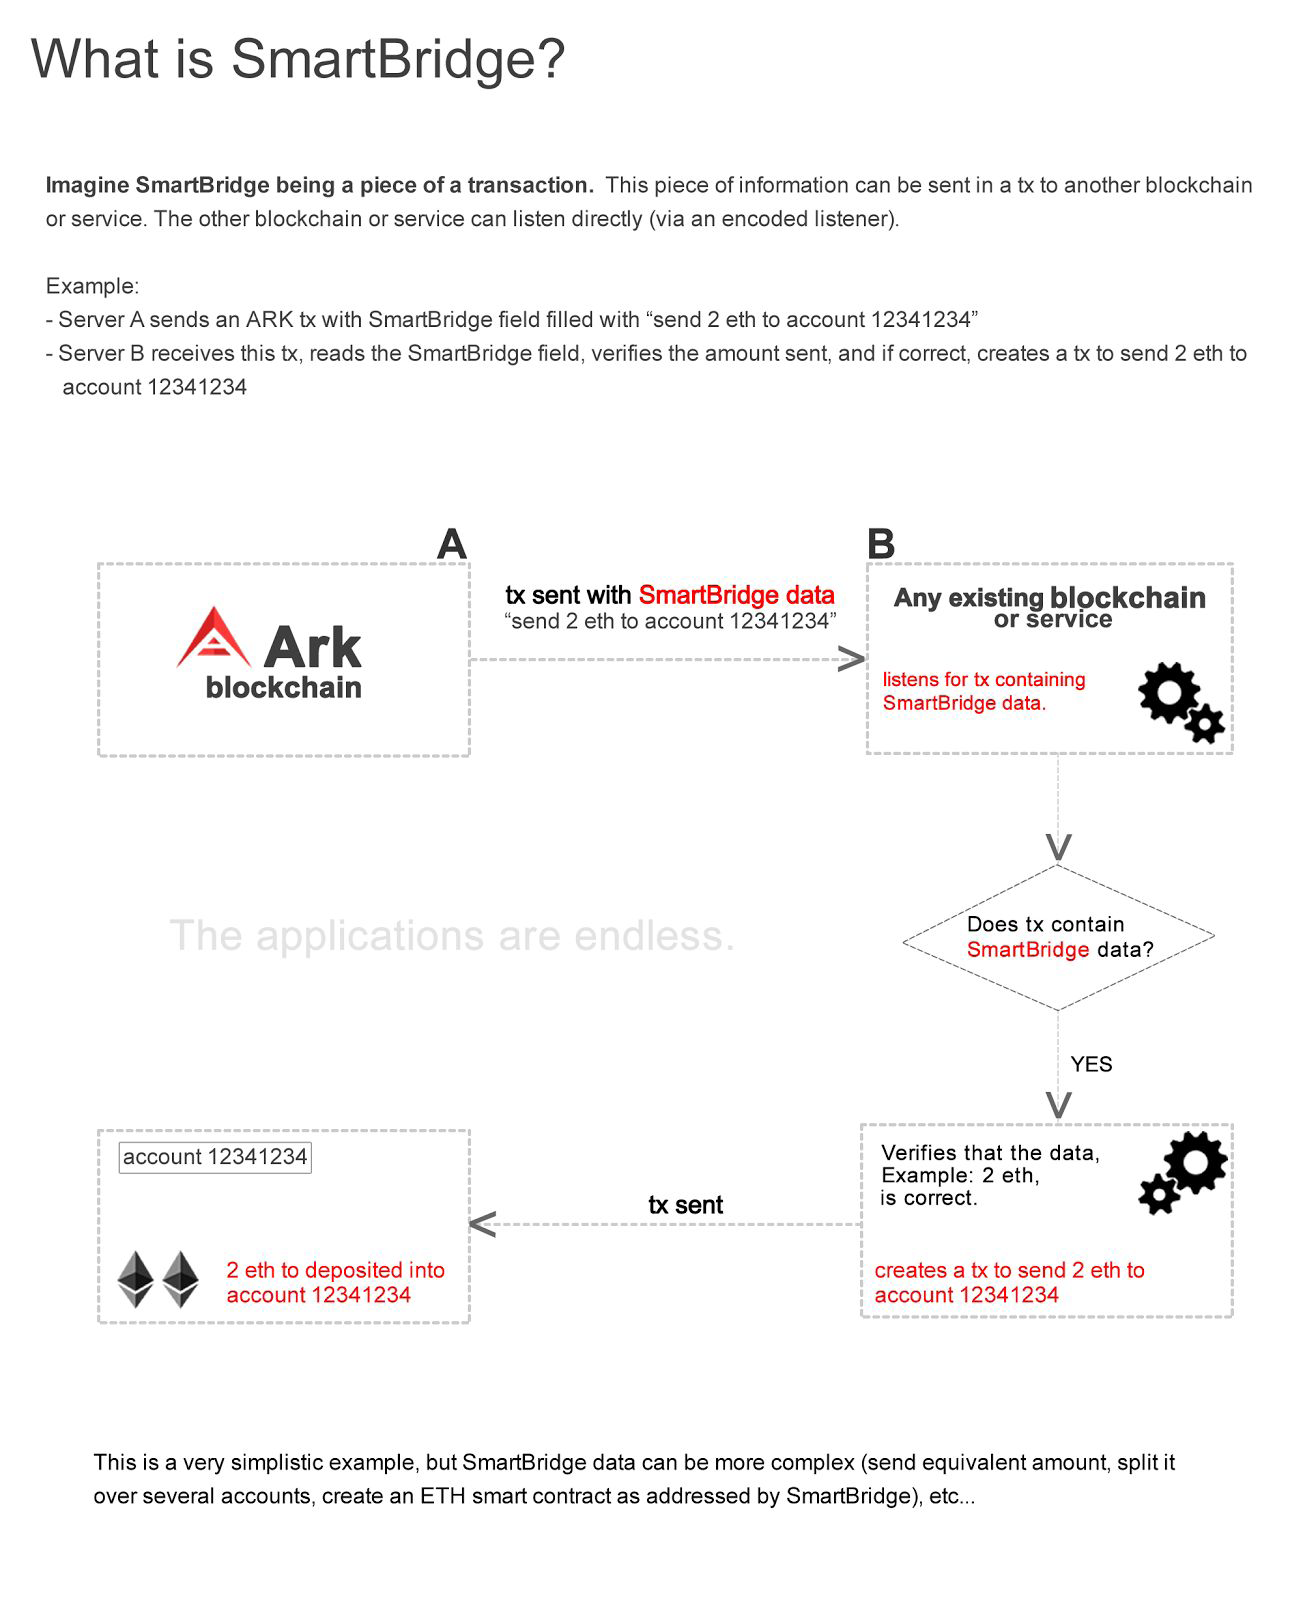
\includegraphics[width=\textwidth,height=\textheight,keepaspectratio]{ARKSmartBridge}
	\captionof{figure}{ARK SmartBridge Technology}
\end{center}

\subsubsection{A.C.E.S. - ARK Contract Execution Service}
ACES is a blockchain interoperability platform that provides simple protocols and tools for building a robust blockchain 
service marketplace.

ACES is composed mainly of the following three components:
\begin{itemize}
	\item \textbf{Listeners} ACES Listeners provide a way for all the different blockchain transaction events to be easily 
	consumed via a common REST-ful API. The API allows consumers to create subscriptions and receive blockchain events 
	in real-time using Webhook callbacks.
	\item \textbf{Services} ACES Services create and execute Service Contracts, which can be anything from uploading 
	a file to a storage blockchain, performing value transfers, creating smart contracts, executing code on 
	blockchain based computing platforms, or interacting with IoT hardware.
	\item \textbf{Marketplace Console} The ACES Marketplace Console is a consumer dashboard for searching and executing 
	service contracts listed on the Marketplace. ACES Service providers can list their service nodes using the Marketplace API.
\end{itemize}

\begin{center}
	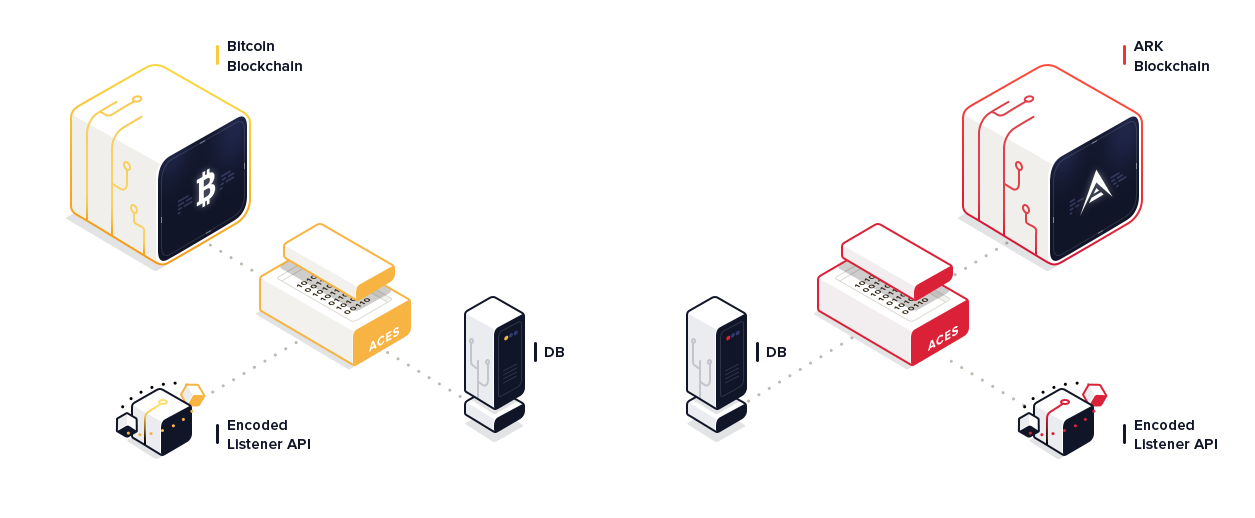
\includegraphics[width=\textwidth,height=\textheight,keepaspectratio]{ACES}
	\captionof{figure}{ARK-BTC A.C.E.S. SmartBridge Implementation Overview}
\end{center}

\subsection{Ripa Liquidity Service Provider (R.L.S.P)}
Using the SmartBridge technology RipaEx will build a mechanism to share liquidity between all the exchanges in the Ripa network
by writing the single exchange orderbook in the Ripa Blockchain and by executing order matching between all exchanges in the network.

In this way you can have the benefits of a decentralized orderbook (like liquidity) with the benefits of a centralized exchange (like
platinum customer support and FIAT exchange).

\subsection{Ripa Community Fund}
To permits the birth of new exchanges in the Ripa network a Ripa Community Fund - RCF - is created with the following characteristics:
\begin{itemize}
	\item \textbf{Starting Principal}: the RCF will have a starting operating capital of 5\% (5,750,000 \PHP) of the genesis block
	\item \textbf{Recurring Participation}: each delegate will contribute to the RCF with 5\% of its forged XPXs
\end{itemize}
\vspace{5mm}
To obtain funds from the RCF to start your own Ripa Exchange you will submit your proposal in the official RCF section in the Ripa forum at
anytime after the first Ripa Exchange instance will be operational.

%----------------------------------------------------------------------------------------
%	CHAPTER 5: Token Sale
%----------------------------------------------------------------------------------------

\chapterimage{chapter_head_4_Dubai.jpg} % Chapter heading image
\chapter{Token Sale}
\section{Introduction}
The RipaEx XPX token sale will be separated into two phases:
	\begin{itemize}
		\item \textbf{\textsc{PreSale}}: that will run from April to June 2018
		\item \textbf{\textsc{RIPA TEC}}: that will run from July to December 2018
	\end{itemize}
\vspace{5mm}
You can easily refer to both phases PreSale and RIPA TEC as \textit{RipaEx ICO}.

\subsection{RIPA TEC}
Fund-raising through the RIPA TEC platform will follow the schedule:
\begin{itemize}
	\item \textcolor{airforceblue}{\textbf{\textit{Exchange} from 07/02/2018 to 07/15/2018}}: at the rate of \PHP/\euro0.0500 (\textcolor{airforceblue}{\textbf{100\% bonus}})
	\item \textcolor{darkgoldenrod}{\textbf{\textit{Cooling-OFF} from 07/16/2018 to 07/22/2018}}: 
	at the rate of \PHP/\euro0.05128205 (\textcolor{darkgoldenrod}{\textbf{95\% bonus}})
	\item \textcolor{airforceblue}{\textbf{\textit{Exchange} from 07/23/2018 to 08/05/2018}}: at the rate of \PHP/\euro0.05714286 (\textcolor{airforceblue}{\textbf{75\% bonus}})
	\item \textcolor{darkgoldenrod}{\textbf{\textit{Cooling-OFF} from 08/06/2018 to 08/12/2018}}: 
	at the rate of \PHP/\euro0.05847953 (\textcolor{darkgoldenrod}{\textbf{71\% bonus}})
	\item \textcolor{airforceblue}{\textbf{\textit{Exchange} from 08/13/2018 to 08/26/2018}}: at the rate of \PHP/\euro0.06666667 (\textcolor{airforceblue}{\textbf{50\% bonus}})
	\item \textcolor{darkgoldenrod}{\textbf{\textit{Cooling-OFF} from 08/27/2018 to 09/02/2018}}: 
	at the rate of \PHP/\euro0.06802721 (\textcolor{darkgoldenrod}{\textbf{47\% bonus}})
	\item \textcolor{airforceblue}{\textbf{\textit{Exchange} from 09/03/2018 to 09/16/2018}}: at the rate of \PHP/\euro0.07142857 (\textcolor{airforceblue}{\textbf{40\% bonus}})
	\item \textcolor{darkgoldenrod}{\textbf{\textit{Cooling-OFF} from 09/17/2018 to 09/23/2018}}: 
	at the rate of \PHP/\euro0.07246377 (\textcolor{darkgoldenrod}{\textbf{38\% bonus}})
	\item \textcolor{airforceblue}{\textbf{\textit{Exchange} from 09/24/2018 to 10/07/2018}}: at the rate of \PHP/\euro0.07692308 (\textcolor{airforceblue}{\textbf{30\% bonus}})
	\item \textcolor{darkgoldenrod}{\textbf{\textit{Cooling-OFF} from 10/08/2018 to 10/14/2018}}: 
	at the rate of \PHP/\euro0.07751938 (\textcolor{darkgoldenrod}{\textbf{29\% bonus}})
	\item \textcolor{airforceblue}{\textbf{\textit{Exchange} from 10/15/2018 to 10/28/2018}}: at the rate of \PHP/\euro0.08333333 (\textcolor{airforceblue}{\textbf{20\% bonus}})
	\item \textcolor{darkgoldenrod}{\textbf{\textit{Cooling-OFF} from 10/29/2018 to 11/04/2018}}: 
	at the rate of \PHP/\euro0.08403361 (\textcolor{darkgoldenrod}{\textbf{19\% bonus}})
	\item \textcolor{airforceblue}{\textbf{\textit{Exchange} from 11/05/2018 to 11/18/2018}}: at the rate of \PHP/\euro0.09090909 (\textcolor{airforceblue}{\textbf{10\% bonus}})
	\item \textcolor{darkgoldenrod}{\textbf{\textit{Cooling-OFF} from 11/19/2018 to 11/25/2018}}: 
	at the rate of \PHP/\euro0.09174312 (\textcolor{darkgoldenrod}{\textbf{9\% bonus}})
	\item \textcolor{airforceblue}{\textbf{\textit{Exchange} from 11/26/2018 to 12/09/2018}}: at the rate of \PHP/\euro0.0952381 (\textcolor{airforceblue}{\textbf{5\% bonus}})
	\item \textcolor{darkgoldenrod}{\textbf{\textit{Cooling-OFF} from 12/09/2018 to 12/16/2018}}: 
	at the rate of \PHP/\euro0.09615385 (\textcolor{darkgoldenrod}{\textbf{4\% bonus}})
\end{itemize}
\vspace{5mm}
Coins distribution will be available at the end of each trading day and performed automatically through the RIPA TEC platform. Minimum
threshold to reach is 25 BTC.\\

\textsc{As the XPX exchange rate is calculated against the euro currency directly you are guaranteed to not loose any invested fund
during the sale period as the XPX tokens will be listed on our exchanges at the beginning of 2019 directly with the same \textbf{\PHP/\euro0.10}
exchange rate agreed during the token sale-ICO phase}.\\

RIPA TEC platform will be available at the following link after July 2018:
\begin{center}
	\href{https://tec.ripaex.io}{\textsc{tec.ripaex.io}}
\end{center}
follow us on Facebook, Twitter, 
\href{https://t.me/ripaex}{Telegram}, 
\href{https://join.slack.com/t/ripaex/shared_invite/enQtMzM4NzUwNjU4OTQ0LTY3MDJmMTdhYTNlZjJlNGUxNzM1YjUwYjgyYjZlMDJmOTg3NTIzNThmNTYyMGQ3ODBkOTRmYzk3Y2Y4MzBkOTY}{Slack}
and all of our official social channel to know when RIPA TEC is starting!!

\section{XPX Ripa Token Distribution}
\textbf{115,000,000} XPX tokens are seeded into the genesis block: distribution of the XPX tokens generated are described into
figure \ref{fig:distribution} and table \ref{tab:distribution}.

\vspace{5mm}
	\begin{tikzpicture}
		\pie [rotate = 180, explode={0.2, 0.1, 0.1, 0.1, 0.1, 0.1}, radius = 3]
		{65/PreSale \& RIPA TEC,
		15/RIPA Founders Team, 
		6/for marketing,
		5/for bounties,
		5/for RCF,
		4/Ark.io SCIC}
	\end{tikzpicture}
	\captionof{figure}{Ripa token distribution}	
	\label{fig:distribution}

\vspace{5mm}
\begin{table}[H]
	\centering
	\begin{tabular}{l l l}
		\toprule
		\textbf{Percentage (\%)} & \textbf{Quantity (\PHP)} & \textbf{Purpose} \\
		\midrule
		65		& 74,750,000	& to distribute in PreSale and RIPA TEC	\\
		15      & 17,250,000	& to RIPA Founders Team	\\
		6       & 6,900,000		& for marketing	\\
		5       & 5,750,000 	& for bounties	\\
		5       & 5,750,000		& for Ripa Community Fund - RCF	\\
		4       & 4,600,000		& to Ark.io SCIC \\
		\bottomrule
	\end{tabular}
	\captionof{table}{Ripa token distribution}
	\label{tab:distribution}
\end{table}

\vspace{5mm}
\textbf{Tokens not sold during the phases of PreSale and RIPA TEC will be burnt} forever to permits and equal distributions 
of the funds and avoid speculations on the token remaining.

\section{Division of Funds}
The funds collected during the PreSale and RIPA TEC phases will be divided as explained in figure \ref{fig:division} and 
table \ref{tab:division} below

\vspace{5mm}
\begin{tikzpicture}
	\pie [rotate = 180, explode={0.2, 0.1, 0.1}, radius = 3]
	{60/for project development,
	20/for marketing, 
	20/for legal support}
\end{tikzpicture}
\captionof{figure}{Ripa division of funds}	
\label{fig:division}

\vspace{5mm}
\begin{table}[H]
	\centering
	\begin{tabular}{l l}
		\toprule
		\textbf{Percentage (\%)} & \textbf{Purpose} \\
		\midrule
		60		& for project development	\\
		20		& for marketing	\\
		20		& for legal support	\\
		\bottomrule
	\end{tabular}
	\captionof{table}{Division of funds}
	\label{tab:division}
\end{table}

\vspace{5mm}
where the row ``for project development'' funds allocation is described in table \ref{tab:focus} below.

\vspace{5mm}
\begin{table}[H]
	\centering
	\begin{tabular}{l l}
		\toprule
		\textbf{Percentage (\%)} & \textbf{Purpose} \\
		\midrule
		50		& functional analysis, technical analysis, development, testing	\\
		20		& technical support	\\
		15		& infrastructure	\\
		10		& security	\\
		5		& analytics	\\
		\bottomrule
	\end{tabular}
	\captionof{table}{Project development focus}
	\label{tab:focus}
\end{table}

%----------------------------------------------------------------------------------------
%	CHAPTER 6: Economic Projections
%----------------------------------------------------------------------------------------

\chapterimage{chapter_head_6_Frankfurt.jpg} % Chapter heading image

\chapter{Business Model}

\section{Project Milestones}
Following the matrix of development per area of interest based on the funds collected during the phases of PreSale and RIPA TEC:
\begin{tcbraster}[raster columns=5,raster rows=1,raster height=0.8cm,
	valign=center, halign=center,
	enhanced,size=small,sharp corners,colframe=azure(colorwheel),coltext=white,
	colback=azure(colorwheel),fit algorithm=hybrid* ]
	\tcboxfit{}
	\tcboxfit{\textbf{25 BTC}}
	\tcboxfit{\textbf{50 BTC}}
	\tcboxfit{\textbf{250 BTC}}
	\tcboxfit{\textbf{1000 BTC}}
\end{tcbraster}
\begin{tcbraster}[raster columns=5,raster rows=4,raster height=10cm,
	valign=center, halign=center,
	enhanced,size=small,sharp corners,colframe=silver,coltext=black,
	colback=silver,fit algorithm=hybrid* ]
	\tcboxfit{\textsc{\textbf{Development}}}
	\tcboxfit{\tcbfontsize{0.8} CRYPTO $\Leftrightarrow$ CRYPTO exchange release with 25 cryptocurrencies supported and 3 main trading pairs}
	\tcboxfit{\tcbfontsize{0.8} CRYPTO $\Leftrightarrow$ FIAT exchange release with MasterCard prepaid card. 50 cryptocurrencies supported and 3 main trading pairs}
	\tcboxfit{\tcbfontsize{0.8} Advanced trading features. Open of a second and third Ripa Exchanges to join the Ripa network}
	\tcboxfit{\tcbfontsize{0.8} Open of ten Ripa Exchanges across the globe}

	\tcboxfit{\textsc{\textbf{Marketing}}}
	\tcboxfit{\tcbfontsize{0.8} Support from one agency, adv campaigns on targeted channels}
	\tcboxfit{\tcbfontsize{0.8} Support from two agencies, adv campaigns pushing harder, store with RipaEx gadgets}
	\tcboxfit{\tcbfontsize{0.8} International presentation event in London}
	\tcboxfit{\tcbfontsize{0.8} Support from five agencies, targeting all UN countries, presentation event in Tokyo}

	\tcboxfit{\textsc{\textbf{Legal}}}
	\tcboxfit{\tcbfontsize{0.8} Legal department working on AML/KYC international standards}
	\tcboxfit{\tcbfontsize{0.8} Legal departments working on AML/KYC international standards in various locations around the Globe}
	\tcboxfit{\tcbfontsize{0.8} Open of office in New York}
	\tcboxfit{\tcbfontsize{0.8} Open of office in Tokyo, intergovernmental parnership for defining AML/KYC standards}

	\tcboxfit{\textsc{\textbf{Blockchain}}}
	\tcboxfit{\tcbfontsize{0.8} DevNET development for RLSP and future ARK releases}
	\tcboxfit{\tcbfontsize{0.8} Contributions to ARK development for AVM}
	\tcboxfit{\tcbfontsize{0.8} Contributions to ARK development for standard timing releases}
	\tcboxfit{\tcbfontsize{0.8} Partnership with ARK for blockchain technology developments}
\end{tcbraster}

\section{Local Market Analysis and 5 Years Projection}
Ripa Exchange on its opening at the beginning of next year and for all the year 2019 is to be expected
to have the following operating numbers:
\begin{itemize}
	\item Registered Users: 5,000			%(1,600,000 BitFinex, 40,000 TheRockTrading)
	\item 24/hours Volume: 25 BTC			%(50,000 BTC BitFinex, 100 BTC TheRockTrading)
	\item Monthly Volume: 750 BTC			%(2,000,000 BTC BitFinex, 5,000 BTC TheRockTrading)
\end{itemize}

Given a transaction fee of 0.20\% the revenue for the first year of operation are expected to be in the order of 180 BTC the 
outcome for the years 2 to 5 is expected to be in the rage described in figure \ref{fig:fiveYearsProjection} 
\begin{center}
	\begin{tikzpicture}
		\begin{axis}[
			symbolic x coords={2019, 2020, 2021, 2022, 2023},
			xtick=data,
			ylabel=BTC,
			xlabel=years
		]
			\addplot[ybar,fill=azure(colorwheel)] coordinates {
				(2019, 180)
				(2020, 300)
				(2021, 500)
				(2022, 1000)
				(2023, 2000)
			};
			\addplot+ [
				sharp plot, color=silver, mark=diamond
				] coordinates {
				(2019,180) (2020,300) (2021,500) (2022,1000) (2023,2000)
				};			
		\end{axis}	
	\end{tikzpicture}
	\captionof{figure}{5 years revenue projection}
	\label{fig:fiveYearsProjection}
\end{center}

Depending on the closing value of the RipaEx ICO, the project is to be expected to open N.1 to N.9 others Ripa Exchange in 
the biennium 2019-2020 spreading the use of the Ripa Exchange codebase and the usage of the XPX token associated with the 
Ripa Blockchain making the figure above into account for each single Ripa Exchange installation.

\section{XPX Token Economics}
As explained in section \ref{sec:theRipaBlockchain} the Ripa Blockchain will have its own XPX token (\PHP symbol) that 
will serve the following purposes:
	\begin{enumerate}
		\item to list new cryptocurrencies on Ripa Exchanges
		\item to advertise new projects
		\item to buy RipaEx gadget on RipaEx Store
		\item to pay for the sell of goods \& services on authorized resellers with our RipaEx POS (Point of Sale)
		\item to share liquidity between Ripa Exchanges in the same network
	\end{enumerate}
It is our main purpose that the economy of the XPX token will stay healthy for all the duration of the RipaEx project for 
this reason we will apply economic strategies\footnote{Like burning tokens not covered from ICO funds} 
to the token economy to make the price of the token rise constantly during all the duration of the project and beyond.


%----------------------------------------------------------------------------------------
%	CHAPTER 7: Conclusion
%----------------------------------------------------------------------------------------

\chapterimage{chapter_head_7_LosAngeles.jpg} % Chapter heading image

\chapter{Team \& Conclusion}

\section{Team}
\begin{tcbraster}[raster columns=1,raster rows=1,raster height=0.4cm,
	valign=center, halign=center,
	enhanced,size=small,sharp corners,colframe=azure(colorwheel),coltext=white,
	colback=azure(colorwheel),fit algorithm=hybrid* ]
	\tcboxfit{}
\end{tcbraster}
\begin{tcbraster}[raster columns=2,raster rows=4,raster height=10cm,
	valign=center, halign=left,
	enhanced,size=small,sharp corners,colframe=silver,coltext=black,
	colback=silver,fit algorithm=hybrid* ]
	\tcboxfit{\tcbfontsize{0.8} \textbf{Giovanni Silvestri @ BitNow}\\
	\textsc{Founder and CEO}\\
	10+ years experience in IT field,\\
	4+ years in cryptocurrencies consultancy and exchanging,\\
	2+ years experience in finance,\\
	Location: Treviso (TV), Italy\\
	\href{https://bitcointalk.org/index.php?action=profile;u=497151;sa=summary}{\faBitcoin}
	\href{https://www.linkedin.com/in/zackko/}{\faLinkedin}
	\href{https://t.me/BitNow}{\faSend}}
	\tcboxfit{\tcbfontsize{0.8} \textbf{Antonello Arena @Darkital}\\
	\textsc{Founder and CFO}\\
	10+ years experience in economics and finance,\\
	4+ years in cryptocurrencies consultancy and exchanging,\\
	Location: Potenza (PO), Italy\\
	\href{https://www.linkedin.com/in/antonello-arena-a26b60b7/}{\faLinkedin}
	\href{https://t.me/darkital}{\faSend}}

	\tcboxfit{\tcbfontsize{0.8} \textbf{Giorgio Isola @isolagio}\\
	\textsc{Founder and CDO}\\
	10+ years experience in design,\\
	4+ years in cryptocurrencies consultancy and exchanging,\\
	Location: Milan (MI), Italy\\
	\href{https://bitcointalk.org/}{\faBitcoin}
	\href{https://www.linkedin.com/}{\faLinkedin}
	\href{https://t.me/isolagio}{\faSend}}
	\tcboxfit{\tcbfontsize{0.8} \textbf{Propose your NAME here}\\
	\textsc{CSO}\\
	3+ years experience in IT networking,\\
	1+ years in network security,\\
	1+ years experience in finance and or cryptocurrencies,\\
	Location: \\
	\href{https://bitcointalk.org/}{\faBitcoin}
	\href{https://www.linkedin.com/}{\faLinkedin}
	\href{https://t.me/}{\faSend}}

	\tcboxfit{\tcbfontsize{0.8} \textbf{Luca Dordolo @gavrilobtc}\\
	\textsc{Advisor}\\
	5+ years in cryptocurrencies consultancy and exchanging,\\
	Location: Udine (UD), Italy\\
	\href{https://bitcointalk.org/index.php?topic=327894.0}{\faBitcoin}
	\href{http://www.gavrilobtc.it/}{\faRss}
	\href{https://t.me/gavrilobtc}{\faSend}}
	\tcboxfit{\tcbfontsize{0.8} \textbf{Adriatic Crypto Hub}\\
	\textsc{Advisor}\\
	5+ years experience in advisoring\\
	5+ years in cryptocurrencies consultancy and exchanging,\\
	Location: Pescara (PE), Italy\\
	\href{https://adriaticrypto.org/}{\faRss}
	\href{https://bitcointalk.org/index.php?topic=2196282.0}{\faBitcoin}
	\href{https://www.linkedin.com/company/adriatic-crypto-hub}{\faLinkedin}
	\href{https://t.me/AdriaCryptoHub}{\faSend}}

	\tcboxfit{\tcbfontsize{0.8} \textbf{Freewillynow}\\
	\textsc{community manager America}\\
	2+ years experience in community management,\\
	5+ years experience in cryptocurrencies,\\
	Location: The Netherlands\\
	\href{https://t.me/freewillynow}{\faSend}}
	\tcboxfit{\tcbfontsize{0.8} \textbf{OnlyTrifiz}\\
	\textsc{community manager EMEA 1/2}\\
	2+ years experience in community management,\\
	5+ years experience in cryptocurrencies,\\
	Location: Italy\\
	\href{https://bitcointalk.org/index.php?action=profile;u=993136}{\faBitcoin}
	\href{https://www.linkedin.com/in/simone-trifiletti/}{\faLinkedin}
	\href{https://t.me/OnlyTrifiz}{\faSend}}

	\tcboxfit{\tcbfontsize{0.8} \textbf{Bitmyst}\\
	\textsc{community manager EMEA 2/2}\\
	2+ years experience in community management,\\
	5+ years experience in cryptocurrencies,\\
	Location: Italy\\
	\href{https://t.me/Bitmyst}{\faSend}}
	\tcboxfit{\tcbfontsize{0.8} \textbf{Warren Rogers @wazzy}\\
	\textsc{community manager Africa - Asia}\\
	2+ years experience in community management,\\
	5+ years experience in cryptocurrencies,\\
	5+ years experience in IT,\\
	Location: Czech Republic\\
	\href{https://www.linkedin.com/in/warren-rogers-8721a069/}{\faLinkedin}
	\href{https://t.me/Wazzy}{\faSend}}

	\tcboxfit{\tcbfontsize{0.8} \textbf{Goose}\\
	\textsc{Developer - Delegate}\\
	1+ years experience in DPOS delegation,\\
	8+ years experience in finance and or cryptocurrencies,\\
	Location: United States \\
	\href{https://bitcointalk.org/index.php?action=profile;u=1122579}{\faBitcoin}
	\href{https://t.me/Delegate_Goose}{\faSend}}
	\tcboxfit{\tcbfontsize{0.8} \textbf{Pimoussefrnl}\\
	\textsc{Delegate}\\
	4+ years experience in DPOS delegation,\\
	\href{https://t.me/pimoussefrnl}{\faSend}}

	\tcboxfit{\tcbfontsize{0.8} \textbf{Bluedragon}\\
	\textsc{Delegate}\\
	2+ years experience in DPOS delegation,\\
	5+ years experience in marketing,\\
	Location: United Kingdom\\
	\href{https://t.me/bluedragon555}{\faSend}}
	\tcboxfit{\tcbfontsize{0.8} \textbf{Toons}\\
	\textsc{Developer - Delegate}\\
	10 years of experience in python development,\\
	3 years of experience in structure design,\\
	2+ years experience in DPOS delegation and cryptocurrencies\\
	\href{https://t.me/}{\faSend}}

	\tcboxfit{\tcbfontsize{0.8} \textbf{BitSnapp}\\
	\textsc{Delegate}\\
	5+ years experience in software development,\\
	2+ years experience in DPOS delegation\\
	Location: Italy\\
	\href{https://bitsnapp.com/}{\faRss}
	\href{https://t.me/giamme1}{\faSend}}
	\tcboxfit{\tcbfontsize{0.8} \textbf{Amol}\\
	\textsc{Developer - Delegate}\\
	1+ years experience Computer Engineering,\\
	1+ years experience in DPOS delegation and cryptocurrencies\\
	Location: Ahmedabad, India\\
	\href{https://twitter.com/mrheisenberger}{\faTwitter}
	\href{https://www.linkedin.com/in/amoltangade}{\faLinkedin}
	\href{https://t.me/dhokala}{\faSend}}

	\tcboxfit{\tcbfontsize{0.8} \textbf{Gandalf}\\
	\textsc{Developer - Delegate}\\
	5+ years experience in software development,\\
	1+ years experience in DPOS delegation\\
	Location: United States\\
	\href{https://t.me/crypto_gandalf}{\faSend}}	
	\tcboxfit{\tcbfontsize{0.8} \textbf{Nick\_Bold}\\
	\textsc{Developer - Delegate}\\
	10+ years experience in software development,\\
	1+ years experience in DPOS delegation\\
	Location: Italy\\
	\href{https://t.me/Nick_Bold}{\faSend}}

	\tcboxfit{\tcbfontsize{0.8} \textbf{gobled}\\
	\textsc{Developer - Delegate}\\
	10+ years experience in software development,\\
	1+ years experience in DPOS delegation\\
	Location: Italy\\
	\href{https://t.me/gobled}{\faSend}}
	\tcboxfit{\tcbfontsize{0.8} \textbf{Propose your NAME here}\\
	\textsc{Developer - Delegate}\\
	1+ years experience in DPOS delegation,\\
	1+ years experience in cryptocurrencies\\
	Location:\\
	\href{https://twitter.com/}{\faTwitter}
	\href{https://www.linkedin.com/}{\faLinkedin}
	\href{https://t.me/}{\faSend}}
\end{tcbraster}

\section{Recommendations}
If you are planning to start your own crypto asset marketplace you are invited to follow the following procedure to make
your start-up plan a success in the Ripa ecosystem:
\begin{enumerate}
	\item Submit your proposal to Ripa Community Fund by its official website\footnote{Available after March 2019} or by contacting us
	on our official social channels
	\item Get the funds you need from RCF, Venture Capital or ICO
	\item Decide the functional specifications of your exchange
	\item Implement the exchange
	\item Open to public
\end{enumerate}

Following the procedure above you are likely to start a successful exchange for which you own the source code and which will 
generate revenues for your business action in the next 5 years.

It can't be stressed enough that if your intent is to open a FIAT $\Leftrightarrow$ CRYPTO exchange you should
focus first on law compliance by studying the AML/KYC laws of the country of incorporation and
finding banking partners to work with. Local financial Authority can help to comply with rules \& regulations and 
local cryptocurrencies foundations can help you to tune your exchanges operations to perform targeted
operations based on the customers interests in the country of incorporation promoting 
cryptocurrency-friendly users in the area of interest.\\

Remember that \textbf{\textsc{running an exchange is hard}} but we'll give you all the tools to start your entrepreneurship venture
with all you need: source code, liquidity and financing will be available to you from day 1 of your trading operations 
so you can focus on giving platinum customer support, law compliance and partnering with financial institutions 
for the success of your entrepreneurship action.

\textsc{Your success is the success of the Ripa exchange network} and we want to achieve that with hard work and the most advanced
technology in the industry for \textsc{YOU} and for the satisfaction of the Ripa network clients.

\section{Social}
\label{sec:social}
Please \href{https://t.me/ripaex}{join our Telegram} to give us feedback on the whitepaper.\\

To be part of our active community or learn more about what we do:
\begin{itemize}
	\item \textbf{Visit our website} \href{https://www.ripaex.io}{\faHome \hspace{0.2cm} www.ripaex.io} 
	\item \textbf{Join our Telegram} \href{https://t.me/ripaex}{\faSend \hspace{0.2cm} t.me/ripaex}
	\item \textbf{Join our Slack} \href{https://join.slack.com/t/ripaex/shared_invite/enQtMzM4NzUwNjU4OTQ0LTY3MDJmMTdhYTNlZjJlNGUxNzM1YjUwYjgyYjZlMDJmOTg3NTIzNThmNTYyMGQ3ODBkOTRmYzk3Y2Y4MzBkOTY}{\faSlack \hspace{0.2cm} ripaex.slack.com}
	\item \textbf{Follow us on Twitter} \href{https://twitter.com/ripaex}{\faTwitter \hspace{0.2cm} twitter.com/ripaex}
	\item \textbf{Follow us on Facebook} \href{https://www.facebook.com/ripaex}{\faFacebook \hspace{0.2cm} www.facebook.com/ripaex}
	\item \textbf{Send Us an e-mail} \href{mailto:info@ripaex.io}{\faInternetExplorer \hspace{0.2cm} info@ripaex.io}
\end{itemize}



%----------------------------------------------------------------------------------------
%	COPYRIGHT PAGE
%----------------------------------------------------------------------------------------
\newpage
~\vfill
\thispagestyle{empty}

\noindent Copyright \copyright\ 2018 Ripa Founder Team\\ % Copyright notice

\noindent \textsc{Published by Ripa Founder Team}\\ % Publisher

\noindent \textsc{www.ripaex.io}\\ % URL

\noindent Licensed under the MIT License (the ``License''). You may not use this file except in compliance with the License. 
You may obtain a copy of the License at \url{https://opensource.org/licenses/MIT}. Unless required by applicable law or agreed to in writing, 
software distributed under the License is distributed on an \textsc{``as is'' basis, without warranties or conditions of any kind}, 
either express or implied. See the License for the specific language governing permissions and limitations under the License.\\ % License information

\noindent \textit{First printing, March 2018 - version 1.0}\\ % Printing/edition date

\noindent \textit{RipaEx VAT 04927110264 - Treviso (TV) - Italy} % Printing/edition date

\end{document}